% THIS IS SIGPROC-SP.TEX - VERSION 3.1
% WORKS WITH V3.2SP OF ACM_PROC_ARTICLE-SP.CLS
% APRIL 2009
%
% It is an example file showing how to use the 'acm_proc_article-sp.cls' V3.2SP
% LaTeX2e document class file for Conference Proceedings submissions.
% ----------------------------------------------------------------------------------------------------------------
% This .tex file (and associated .cls V3.2SP) *DOES NOT* produce:
%       1) The Permission Statement
%       2) The Conference (location) Info information
%       3) The Copyright Line with ACM data
%       4) Page numbering
% ---------------------------------------------------------------------------------------------------------------
% It is an example which *does* use the .bib file (from which the .bbl file
% is produced).
% REMEMBER HOWEVER: After having produced the .bbl file,
% and prior to final submission,
% you need to 'insert'  your .bbl file into your source .tex file so as to provide
% ONE 'self-contained' source file.
%
% Questions regarding SIGS should be sent to
% Adrienne Griscti ---> griscti@acm.org
%
% Questions/suggestions regarding the guidelines, .tex and .cls files, etc. to
% Gerald Murray ---> murray@hq.acm.org
%
% For tracking purposes - this is V3.1SP - APRIL 2009

\documentclass{acm_proc_article-sp}

\begin{document}

\title{KennySync}
\subtitle{[A Ruby Implementation of Paxos]}
%
% You need the command \numberofauthors to handle the 'placement
% and alignment' of the authors beneath the title.
%
% For aesthetic reasons, we recommend 'three authors at a time'
% i.e. three 'name/affiliation blocks' be placed beneath the title.
%
% NOTE: You are NOT restricted in how many 'rows' of
% "name/affiliations" may appear. We just ask that you restrict
% the number of 'columns' to three.
%
% Because of the available 'opening page real-estate'
% we ask you to refrain from putting more than six authors
% (two rows with three columns) beneath the article title.
% More than six makes the first-page appear very cluttered indeed.
%
% Use the \alignauthor commands to handle the names
% and affiliations for an 'aesthetic maximum' of six authors.
% Add names, affiliations, addresses for
% the seventh etc. author(s) as the argument for the
% \additionalauthors command.
% These 'additional authors' will be output/set for you
% without further effort on your part as the last section in
% the body of your article BEFORE References or any Appendices.

\numberofauthors{3}
%
\author{
% You can go ahead and credit any number of authors here,
% e.g. one 'row of three' or two rows (consisting of one row of three
% and a second row of one, two or three).
%
% The command \alignauthor (no curly braces needed) should
% precede each author name, affiliation/snail-mail address and
% e-mail address. Additionally, tag each line of
% affiliation/address with \affaddr, and tag the
% e-mail address with \email.
%
% 1st. author
\alignauthor
Will Anderson\\
       \affaddr{Rose-Hulman Institute of Technology}\\
       \affaddr{5500 Wabash Ave.}\\
       \affaddr{Terre Haute, IN 47803}\\
       \email{anderswc@rose-hulman.edu}
% 2nd. author
\alignauthor
Tim Ekl\\
       \affaddr{Rose-Hulman Institute of Technology}\\
       \affaddr{5500 Wabash Ave.}\\
       \affaddr{Terre Haute, IN 47803}\\
       \email{ekltl@rose-hulman.edu}
% 3rd. author
\alignauthor
Eric Reed\\
       \affaddr{Rose-Hulman Institute of Technology}\\
       \affaddr{5500 Wabash Ave.}\\
       \affaddr{Terre Haute, IN 47803}\\
       \email{reedec@rose-hulman.edu}
}
\date{18 May 2012}

\maketitle
\begin{abstract}

This paper presents an overview of the Paxos conflict-resolution algorithm,
first described by Leslie Lamport, and a discussion of a Ruby implementation of
the same. Adapting the Paxos algorithm to Ruby 1.9 presented both a challenge
and an opportunity to the authors: though Paxos is of significance in both
industry and the educational community as a leading example of conflict
resolution, it has no widely available implementations in a ``modern''
language, and modeling it on a small scale for demonstrative purposes has its
own benefits and drawbacks.

\end{abstract}

\category{H.2.7}{Database Management}{Database Administration}{security, integrity, and protection}

\terms{Integrity, conflict resolution}

\keywords{Paxos, conflict resolution} % NOT required for Proceedings

\section{Background}

Paxos, originally described in 1998 by Leslie Lamport \cite{paxos}, is a
distributed fault-tolerant algorithm for consistency in decision-making. Lamport
originally released his description of the algorithm in the context of a fictive
Greek society on an island also named Paxos; this was ill-received, leading
Lamport to reduce the algorithm down to a ``simple English'' version
\cite{simple-paxos}.

Both papers describe the same core algorithm, which is framed as a state machine
by Lamport. Individual processes involved in an execution of the Paxos
``protocol'' perform four major actions (and take on roles according to those
actions): they \textit{prepare}, \textit{propose}, \textit{accept}, and
\textit{learn} values. Each node involved in Paxos performs all of these
actions, though the cohort may elect a single ``distinguished'' node for some
actions, speeding the process of reaching consensus.

The Paxos algorithm is notable for the guarantees it provides. With Paxos, the
entire network seeking consensus is assured of ``safety:'' nodes cannot learn
values that were not agreed upon. Furthermore, Paxos also provides a guarantee
of ``progress:'' nodes will eventually reach consensus (under the assumptions
outlined by Lamport).

In the context of data management and integration, these two properties can be
highly useful in decentralized or replicated databases. By implementing Paxos as
a wrapper to database functions, users can be assured that multiple machines all
agree on data to be stored. In addition, users with specialized needs can use
one of the many variants of Paxos available; versions that decrease processing
requirements \cite{cheap-paxos}, run more quickly than the original
\cite{fast-paxos}, and work in a more general case than originally described
\cite{generalized-paxos} all exist.

\section{Implementation}

The authors chose to implement the Paxos algorithm in the Ruby 1.9 programming
language. Ruby, first publicly released in 1995 \cite{about-ruby}, is a dynamic
general-purpose scripting language that has achieved popularity in recent years;
it was chosen for its ease of use, rapid development potential, and wide array
of extension packages (called ``gems'') that aid in development. This
implementation is called KennySync \cite{kennysync}.

KennySync is a command-line application allowing users to instantiate individual
nodes in a Paxos cohort, name each node, and optionally provide textual or
visual feedback about the behavior of the Paxos network involved. In addition,
KennySync supports rudimentary connections to a Redis database as a
proof-of-concept.

The architecture of KennySync is primarily event-driven. As in Lamport's
original description, each instance of KennySync maintains most of its
information as state variables, modifying its internal state in response to
messages it receives from other KennySync instances. The complete set of
messages known to KennySync are listed in Table 1.

\begin{table*}
\centering
\begin{tabular}{l | l}
\textbf{Message} & \textbf{Action/behavior} \\ \hline
\textit{Node} & Informs a KennySync instance of another node's existence; used
to synchronize all instances with each other \\ \hline
\textit{Sync} & Informs a KennySync instance of a newly started node's
unique identifier \\ \hline
\textit{Info} & Provides a simple informational message to a KennySync instance
\\ \hline
\textit{Broadcast} & Sends an informational message to all known KennySync
instances \\ \hline
\textit{Prepare} & Follows Lamport's description:
requests a promise not to accept certain future proposals \\ \hline
\textit{Promise} & Follows Lamport's description:
guarantees that certain future proposals will not be accepted \\ \hline
\textit{AcceptRequest} & Follows Lamport's description: asks another KennySyn
instance to accept a particular value \\ \hline
\textit{Accept} & Follows Lamport's description: informs
another KennySync instance that a given value has been agreed upon \\ \hline
\end{tabular}
\caption{List of message types known to KennySync nodes}
\end{table*}

\subsection{Event Architecture}

The event-driven nature of the KennySync Paxos implementation is supported in
large part by EventMachine, a Ruby gem designed to handle asynchronous message
exchange and event communication between multiple processes. KennySync
encapsulates each of the messages described in Table 1 as its own object; a
rudimentary language parser manufactures instances of these objects as they are
received through EventMachine. Responses are transmitted back using those same
objects, serialized to be transmitted across connections managed by
EventMachine.

In order for maximal interoperability with potential future implementations, as
well as ease of use with EventMachine, the underlying connections across which
messages are transmitted are based on TCP/IP connections. This allows KennySync
to respond to changes in connection status, as well as new messages, through a
common EventMachine-provided interface.

Finally, logging and visualization (if requested) are all handled in a similar
fashion: KennySync ships with a number of ``listeners,'' each of which observes
messages and state changes within a KennySync instance and provides output or
log data based on those events. In this way, KennySync presents a highly
extensible framework for future development or modification; one needs simply to
add a listener or message type with the appropriate method signatures to fully
integrate it into the KennySync application.

\subsection{Message Implementations}

In keeping with the event architecture described above, KennySync implements the
Paxos protocol by responding to individual messages it receives. As such, it
divides Lamport's original Paxos protocol into several executable ``chunks,''
each of which runs upon receipt of the appropriate message type. The start of a
single Paxos run -- the sending of a Prepare message -- is generally triggered
by receiving a value from a user or client program as input. From that point,
the protocol proceeds as described in the following pseudocode chunks. Note that
each chunk receives a message ID (uniquely identifying the particular value in
question) and a value under consideration.

\subsubsection{Prepare Message}

\begin{verbatim}
def prepare(id, value)
  current_proposal_id = id
  if id > highest_promised_id
    highest_promised_id = id
    send_message promise_message(id, highest_accepted_id)
\end{verbatim}

\subsubsection{Promise Message}

For this chunk, note that the Paxos node has already extracted the highest
accepted ID from the promise message sent from the Prepare phase and checked its
validity (via its parsing mechanism); as such, it is replaced here by the actual
value in question.

\begin{verbatim}
def promise(id, value)
  if id == current_proposal_id
    number_acceptances += 1
    append value to acceptances
    if number_acceptances > number_connections / 2
      best_value = best of acceptances
      send_message accept_request_message(id, best_value)
\end{verbatim}

\subsubsection{Accept-Request Message}

\begin{verbatim}
def acceptrequest(id, value)
  if id >= highest_promised_id
    highest_accepted_id = id
    send_message accepted_message(id, value)
\end{verbatim}

\subsubsection{Accepted Message}

\begin{verbatim}
def accepted(id, value)
  accepted_items[id, value] += 1
  if accepted_items[id, value] > number_connections / 2
    output value
    read next_id, next_value from input
    send_message prepare_message(next_id, next_value)
\end{verbatim}

\subsection{Database Support}

In addition to providing a complete implementation of the Paxos protocol,
KennySync also integrates with the open-source key-value store Redis for
persistence of values that reach consensus. When configured properly, KennySync
will flush values that are ``learned'' through a run of the Paxos algorithm to
a local Redis database, which can then be read to ascertain a value in question.
Each KennySync instance is capable of maintaining its own Redis database, making
it possible to use KennySync to synchronize multiple disparate databases.

However, in order to support this persistence mechanism, KennySync makes some
minor changes to the original Paxos protocol. It is a limitation of Lamport's
Paxos that the algorithm reaches consensus on one value only; each new value to
be learned requires a full new run of the Paxos protocol to be completed. (This
is similar to the problem that so-called ``Fast Paxos'' sought to defeat by
persisting a distinguished node across multiple runs \cite{fast-paxos}.)

To avoid this problem, KennySync fully encapsulates the Paxos protocol and
allows users to ``black box'' certain Paxos nodes on program startup. This
provides the ability to input proposed values directly into the black-boxed node
as plain text input, and rely on the node in question to run the value through
the full Paxos protocol. To this end, each node maintains input and output
queues; the input queue receives values from the environment, while the output
queue streams learned values out into a daemon or other external program. In
this way, users can use KennySync as a thin interface between a Redis client and
corresponding database; the user simply relies on Paxos to learn values it
provides and pass them through to the database as required. This architecture is
illustrated in Figure 1.

\begin{figure}
\centering
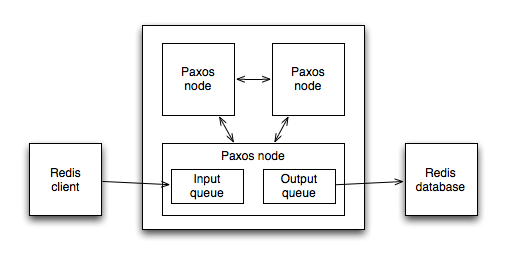
\includegraphics[width=3in]{arch.png}
\caption{Architecture of a KennySync network: clients stream values into a
single node's input queue, allow the network to learn the values, then rely on
the node's output queue to provide those values to a database backend or other
listener program}
\end{figure}

\section{Results}

In its final state, the authors believe KennySync to be a largely bug-free
implementation of the core Paxos protocol. It has been tested and works well in
configurations up to six nodes; with minimal changes, KennySync could support
networks with up to 65,535 nodes on the same machine, or with an arbitrary
number of nodes if distributed across multiple machines. The primary limitation
in this case is the addressing scheme of TCP/IP connections.

Performance-wise, KennySync is presently limited largely by operator
intervention and reaction times. In networks with more than two Paxos nodes,
KennySync requires human responses to complete the entire Paxos protocol; no
automated response criteria are currently implemented, and so KennySync is quite
dependent on its operator for the timing of a single run. In networks of only
two nodes, KennySync achieves a quorum (one node) immediately after proposal,
and so response time is uninteresting in this case.

\section{Conclusions}

Despite the lack of popular implementations ``in the wild'' today, the authors
have shown Paxos to be a viable protocol for conflict resolution in distributed
data-management schemes. Its implementation in Ruby, a language growing rapidly
in popularity, and its connection to Redis both allow for the Paxos protocol to
gain a foothold in the shifting landscape of modern data replication.

\subsection{Future Work}

Though KennySync is a reasonably complete implementation for its modest goals,
there are a number of areas where it could stand to improve. At present, its
primary barrier to widespread acceptance is most likely its stability; as an
academic exercise, KennySync does not focus on the same reliability requirements
that a production use might require of it.

In addition, KennySync could stand to gain a significant amount by becoming
integrated with a broader range of persistent data stores than just Redis;
relational SQL engines, though seeing some slight loss in market share to newer
NoSQL and key-value stores, remain the dominant tool in enterprise data storage.
KennySync would do well to gain a flexible, extensible interface to those types
of database system in the future.

\section{Acknowledgments}

The authors would like to acknowledge Dr. Sriram Mohan of Rose-Hulman Institute
of Technology for his assistance and guidance in the implementation process, and
for setting the challenge of implementing Paxos in the first place. Without him,
KennySync would likely not exist.

In addition, the authors would like to recognize Kenny Gao, a guiding light in
so many students' lives at Rose-Hulman. KennySync is, with the greatest respect
and deference, dedicated to Kenny.

%
% The following two commands are all you need in the
% initial runs of your .tex file to
% produce the bibliography for the citations in your paper.
\bibliographystyle{abbrv}
\bibliography{sigproc}  % sigproc.bib is the name of the Bibliography in this case
% You must have a proper ".bib" file
%  and remember to run:
% latex bibtex latex latex
% to resolve all references
%
% ACM needs 'a single self-contained file'!
%
\balancecolumns
% That's all folks!
\end{document}
